\section{Results}
\label{sec:results}

We organize the presentation of our findings by topic, including how users
\emph{perceive} (\Cref{sec:perception}), \emph{manage} (\Cref{sec:manage}),
and \emph{wish to improve} (\Cref{sec:improve}) onion services.  We interleave the
results from our online survey with our interviews, focusing primarily on our
survey data but bringing up anecdotes and findings from our interviews as
appropriate.

\subsection{User perceptions of onion services}
\label{sec:perception}

\subsubsection{Mental models of Onion Services}
While the work of Tor developers is often held in high esteem, the content that
is hosted on onion services is perceived very differently.  Many of our participants were not able to define what an onion services were, such as one participant who sought clarification: \textquote[P03]{So
it's like the Hidden Wiki and stuff like that, where you can buy drugs and\dots
or supposedly.}

We asked our interview participants to draw sketches of onion services and the Tor network.\footnote{All sketches are available online at
\url{https://nymity.ch/onion-services/mental-models/}.}  All participants drew a
sketch of the Tor network but not all drew onion services because they had not
experienced them. \mc{how many were in each category?}  Interestingly, all participants understood that key to the
Tor network's anonymity is the bouncing of network traffic across several
relays, as evidenced by \Cref{fig:tor-sketch}, drawn by a participant with no
technical background.\footnote{However, the sketch is incorrect in two places: the
number of hops in a Tor circuit is three, and the circuit's forward and reverse
path are identical.} Analogously, most of our participants understood that
network traffic does not leave the Tor network when connecting to onion
services. By contrast, \Cref{fig:os-sketch} illustrates an example of a participants' understanding of an onion serice, again drawn by a
non-technical participant.  The last hop in the circuit is an onion, correctly
suggesting that network traffic does not leave the Tor network, albeit the
number of hops is incorrect.

\begin{figure}[t]
    \centering

    \begin{subfigure}[t]{\linewidth}
        \centering
        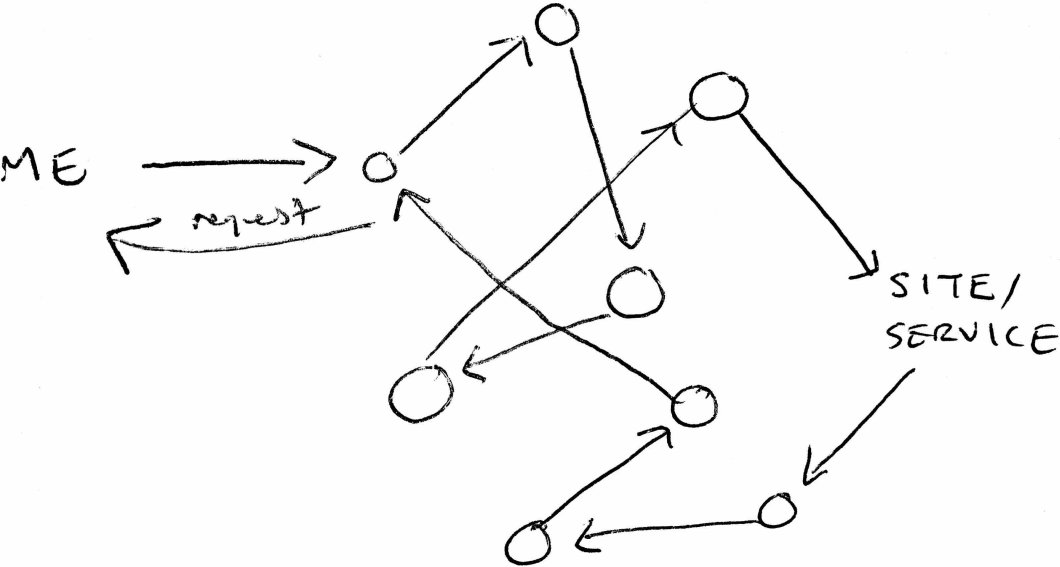
\includegraphics[width=0.8\linewidth]{figures/tor-sketch.jpg}
        \subcaption{A non-technical interview subject's (P08) sketch of how they
        believe the Tor network works.  The participant correctly understands
        the concept of bouncing network traffic over several hops.}
        \label{fig:tor-sketch}
    \end{subfigure}

    \begin{subfigure}[t]{\linewidth}
        \centering
        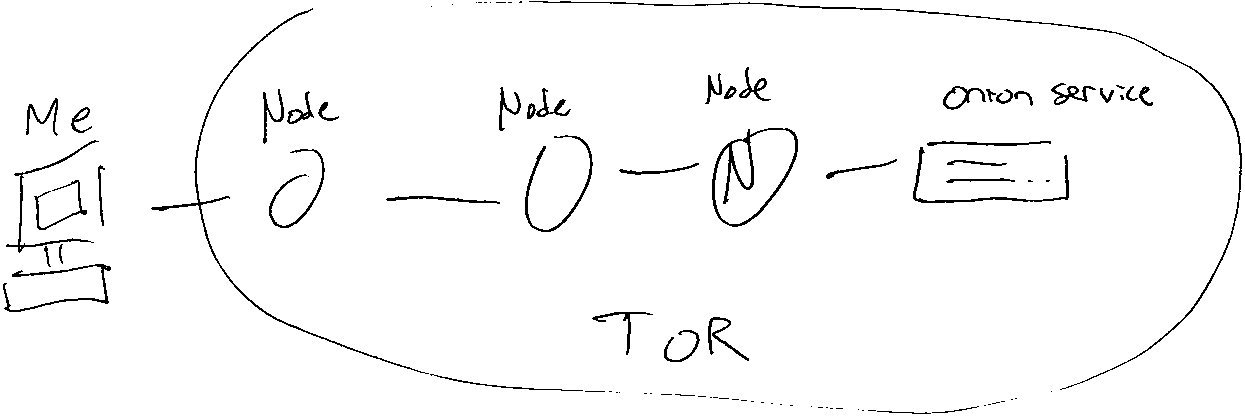
\includegraphics[width=0.8\linewidth]{figures/os-sketch.jpg}
        \subcaption{A non-technical interview subject's (P13) sketch of their
        mental model of an onion service.  Instead of a web site, the final hop
        is another Tor hop.}
        \label{fig:os-sketch}
    \end{subfigure}

    \caption{Sketches of two different, non-technical interview participants of
    how the Tor network works (top) and how onion services work (bottom).}
\end{figure}


We asked our participants what is their perception of Onion Services and according to the majority of our respondents (9/17) these are services that enable the user to access Web content in anonymous manner. Moreover, 3 participants stressed that such protection is not only for visitors but also for people providing these services.
Some of our interviewees did not distinguish disguising their \textsc{ip}
address from disguising their real-world identity and instead used the umbrella
term of ``anonymity'' to refer to both concepts.  This conflation of concepts
paints an incomplete picture of the security and privacy guarantees that the Tor
network provides, further illustrated by one participant's question:
\textquote[P07]{What's the point of going to Facebook using onion services when
their business model is still about collecting your data?}

Many of our \mc{how many} interview participants were unaware of the merit in using Facebook's onion service. For instance, interview participants did not realize that while the company indeed
knows who is logging in, it does not know Tor users' \textsc{ip} address (and
hence location) or operating system.  Moreover, 1 participant (P10) claimed that using onion links may influence the usability of their ‘normal’ corresponding websites – he shared a story in which he postulated that his Facebook account had been flagged for suspicious activity and then was deactivated because he had logged in through Tor browser.  Nevertheless, P10 did not get any explanation from Facebook administrators. On top of that, onion services provide
end-to-end security and self-authenticating names.  Syverson and Boyce took a
step back and looked at how onion services can improve website
authentication~\cite{Syverson2015a}.  These benefits are difficult to convey to
non-technical users, and even experts sometimes advocate an ``all or nothing''
approach to online anonymity, overlooking important nuances.

\subsubsection{Onion Services Do Not Make Users Feel Safer}
In our survey, we asked how safe our
respondents feel when using Tor Browser and onion services, respectively.
\Cref{fig:perceived-security} shows the results.  
86\% of our survey respondents feel at least somewhat safe using Tor Browser as compared to just over two thirds (67\%) of users of onion services.

\begin{figure}[t]
    \centering
    % Created by tikzDevice version 0.10.1 on 2018-01-12 16:35:49
% !TEX encoding = UTF-8 Unicode
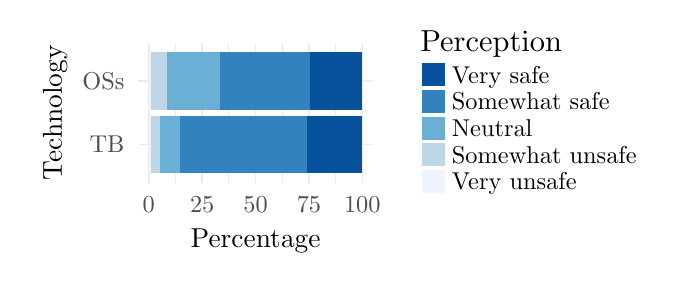
\begin{tikzpicture}[x=1pt,y=1pt]
\definecolor{fillColor}{RGB}{255,255,255}
\path[use as bounding box,fill=fillColor,fill opacity=0.00] (0,0) rectangle (231.26, 86.72);
\begin{scope}
\path[clip] ( 39.91, 30.77) rectangle (124.79, 81.22);
\definecolor{drawColor}{gray}{0.92}

\path[draw=drawColor,line width= 0.3pt,line join=round] ( 53.42, 30.77) --
	( 53.42, 81.22);

\path[draw=drawColor,line width= 0.3pt,line join=round] ( 72.71, 30.77) --
	( 72.71, 81.22);

\path[draw=drawColor,line width= 0.3pt,line join=round] ( 92.00, 30.77) --
	( 92.00, 81.22);

\path[draw=drawColor,line width= 0.3pt,line join=round] (111.29, 30.77) --
	(111.29, 81.22);

\path[draw=drawColor,line width= 0.6pt,line join=round] ( 39.91, 44.53) --
	(124.79, 44.53);

\path[draw=drawColor,line width= 0.6pt,line join=round] ( 39.91, 67.46) --
	(124.79, 67.46);

\path[draw=drawColor,line width= 0.6pt,line join=round] ( 43.77, 30.77) --
	( 43.77, 81.22);

\path[draw=drawColor,line width= 0.6pt,line join=round] ( 63.06, 30.77) --
	( 63.06, 81.22);

\path[draw=drawColor,line width= 0.6pt,line join=round] ( 82.35, 30.77) --
	( 82.35, 81.22);

\path[draw=drawColor,line width= 0.6pt,line join=round] (101.64, 30.77) --
	(101.64, 81.22);

\path[draw=drawColor,line width= 0.6pt,line join=round] (120.93, 30.77) --
	(120.93, 81.22);
\definecolor{fillColor}{RGB}{239,243,255}

\path[fill=fillColor] ( 43.77, 34.21) rectangle ( 44.51, 54.85);
\definecolor{fillColor}{RGB}{189,215,231}

\path[fill=fillColor] ( 44.51, 34.21) rectangle ( 47.92, 54.85);
\definecolor{fillColor}{RGB}{107,174,214}

\path[fill=fillColor] ( 47.92, 34.21) rectangle ( 54.90, 54.85);
\definecolor{fillColor}{RGB}{49,130,189}

\path[fill=fillColor] ( 54.90, 34.21) rectangle (100.90, 54.85);
\definecolor{fillColor}{RGB}{8,81,156}

\path[fill=fillColor] (100.90, 34.21) rectangle (120.93, 54.85);
\definecolor{fillColor}{RGB}{239,243,255}

\path[fill=fillColor] ( 43.77, 57.15) rectangle ( 44.67, 77.78);
\definecolor{fillColor}{RGB}{189,215,231}

\path[fill=fillColor] ( 44.67, 57.15) rectangle ( 50.19, 77.78);
\definecolor{fillColor}{RGB}{107,174,214}

\path[fill=fillColor] ( 50.19, 57.15) rectangle ( 69.60, 77.78);
\definecolor{fillColor}{RGB}{49,130,189}

\path[fill=fillColor] ( 69.60, 57.15) rectangle (101.98, 77.78);
\definecolor{fillColor}{RGB}{8,81,156}

\path[fill=fillColor] (101.98, 57.15) rectangle (120.93, 77.78);
\end{scope}
\begin{scope}
\path[clip] (  0.00,  0.00) rectangle (231.26, 86.72);
\definecolor{drawColor}{gray}{0.30}

\node[text=drawColor,anchor=base east,inner sep=0pt, outer sep=0pt, scale=  0.88] at ( 34.96, 41.50) {TB};

\node[text=drawColor,anchor=base east,inner sep=0pt, outer sep=0pt, scale=  0.88] at ( 34.96, 64.43) {OSs};
\end{scope}
\begin{scope}
\path[clip] (  0.00,  0.00) rectangle (231.26, 86.72);
\definecolor{drawColor}{gray}{0.30}

\node[text=drawColor,anchor=base,inner sep=0pt, outer sep=0pt, scale=  0.88] at ( 43.77, 19.76) {0};

\node[text=drawColor,anchor=base,inner sep=0pt, outer sep=0pt, scale=  0.88] at ( 63.06, 19.76) {25};

\node[text=drawColor,anchor=base,inner sep=0pt, outer sep=0pt, scale=  0.88] at ( 82.35, 19.76) {50};

\node[text=drawColor,anchor=base,inner sep=0pt, outer sep=0pt, scale=  0.88] at (101.64, 19.76) {75};

\node[text=drawColor,anchor=base,inner sep=0pt, outer sep=0pt, scale=  0.88] at (120.93, 19.76) {100};
\end{scope}
\begin{scope}
\path[clip] (  0.00,  0.00) rectangle (231.26, 86.72);
\definecolor{drawColor}{RGB}{0,0,0}

\node[text=drawColor,anchor=base,inner sep=0pt, outer sep=0pt, scale=  0.99] at ( 82.35,  7.44) {Percentage};
\end{scope}
\begin{scope}
\path[clip] (  0.00,  0.00) rectangle (231.26, 86.72);
\definecolor{drawColor}{RGB}{0,0,0}

\node[text=drawColor,rotate= 90.00,anchor=base,inner sep=0pt, outer sep=0pt, scale=  0.99] at ( 12.32, 56.00) {Technology};
\end{scope}
\begin{scope}
\path[clip] (  0.00,  0.00) rectangle (231.26, 86.72);
\definecolor{drawColor}{RGB}{0,0,0}

\node[text=drawColor,anchor=base west,inner sep=0pt, outer sep=0pt, scale=  1.10] at (141.86, 78.11) {Perception};
\end{scope}
\begin{scope}
\path[clip] (  0.00,  0.00) rectangle (231.26, 86.72);
\definecolor{fillColor}{RGB}{8,81,156}

\path[fill=fillColor] (142.58, 65.57) rectangle (150.79, 73.78);
\end{scope}
\begin{scope}
\path[clip] (  0.00,  0.00) rectangle (231.26, 86.72);
\definecolor{fillColor}{RGB}{49,130,189}

\path[fill=fillColor] (142.58, 55.93) rectangle (150.79, 64.15);
\end{scope}
\begin{scope}
\path[clip] (  0.00,  0.00) rectangle (231.26, 86.72);
\definecolor{fillColor}{RGB}{107,174,214}

\path[fill=fillColor] (142.58, 46.30) rectangle (150.79, 54.51);
\end{scope}
\begin{scope}
\path[clip] (  0.00,  0.00) rectangle (231.26, 86.72);
\definecolor{fillColor}{RGB}{189,215,231}

\path[fill=fillColor] (142.58, 36.66) rectangle (150.79, 44.87);
\end{scope}
\begin{scope}
\path[clip] (  0.00,  0.00) rectangle (231.26, 86.72);
\definecolor{fillColor}{RGB}{239,243,255}

\path[fill=fillColor] (142.58, 27.03) rectangle (150.79, 35.24);
\end{scope}
\begin{scope}
\path[clip] (  0.00,  0.00) rectangle (231.26, 86.72);
\definecolor{drawColor}{RGB}{0,0,0}

\node[text=drawColor,anchor=base west,inner sep=0pt, outer sep=0pt, scale=  0.88] at (153.31, 66.65) {Very safe};
\end{scope}
\begin{scope}
\path[clip] (  0.00,  0.00) rectangle (231.26, 86.72);
\definecolor{drawColor}{RGB}{0,0,0}

\node[text=drawColor,anchor=base west,inner sep=0pt, outer sep=0pt, scale=  0.88] at (153.31, 57.01) {Somewhat safe};
\end{scope}
\begin{scope}
\path[clip] (  0.00,  0.00) rectangle (231.26, 86.72);
\definecolor{drawColor}{RGB}{0,0,0}

\node[text=drawColor,anchor=base west,inner sep=0pt, outer sep=0pt, scale=  0.88] at (153.31, 47.37) {Neutral};
\end{scope}
\begin{scope}
\path[clip] (  0.00,  0.00) rectangle (231.26, 86.72);
\definecolor{drawColor}{RGB}{0,0,0}

\node[text=drawColor,anchor=base west,inner sep=0pt, outer sep=0pt, scale=  0.88] at (153.31, 37.74) {Somewhat unsafe};
\end{scope}
\begin{scope}
\path[clip] (  0.00,  0.00) rectangle (231.26, 86.72);
\definecolor{drawColor}{RGB}{0,0,0}

\node[text=drawColor,anchor=base west,inner sep=0pt, outer sep=0pt, scale=  0.88] at (153.31, 28.10) {Very unsafe};
\end{scope}
\end{tikzpicture}

    \caption{The level of safety our respondents perceive when using Tor
    Browser (\textsc{tb}) and onion services (\textsc{os}s).}
    \label{fig:perceived-security}
\end{figure}

Our survey responses indicated that our participants, many of whom were non-experts, lacked the ability to evaluate (or even understand) the
Tor network's design which is why they defer to expert opinion, their gut
feeling, or the trust they place in Tor developers.  With respect to onion
services, the majority of survey respondents expressed that the added security and anonymity makes
them feel safe.  Another factor contributing to the perceived security is that
advertising companies are nowhere near as present on onion services as they are
on the web.  Orthogonal to the technology, many participants voiced concern
about illegal and questionable content on onion services, described by some as a
``Wild West.'' Phishing sites, honeypots, and compromised onion sites further
contribute to this perception.

Although our interviewees tended to evaluate Onion links as safer than corresponding websites (8 vs. 4 participants), 6 people stressed that you need to be careful while using OS, as P13 shared with us: “You can compromise endpoints, I know we've seen cases where people have visited onion services that aren't particularly well protected. Sure, you're visiting a service that is technically only existing within the Tor network, but perhaps it's leaking some information that allows people to then find the location of the server and use that to derive people's identities.”. 

\subsubsection{Onion Services Used For Purposes Other Than Web Browsing}
In the survey, we asked about how often our respondents browse onion
services.  The usage frequency was almost uniformly distributed among our survey
respondents; 24\% use onion sites less than once a month, 22\% use them about
monthly, 25\% weekly, and 23\% daily.  The remaining 6\% has never used an onion
service before.

The majority of our survey respondents (61.8\%) had used onion services for purposes
other than web browsing before.  Several protocols, such as the chat application
Ricochet~\cite{ricochet} and the file sharing application
OnionShare~\cite{onionshare}, were purpose-built on top of onion services while
existing \textsc{tcp}-based tools, such as \textsc{ssh}, can transparently use
onion addresses instead of traditional \textsc{ip} addresses.  Almost one third
(29.7\%) of our participants used onion services for non-browsing activities at
least once a week. \mc{do we know what these were?}

The majority of our survey participants  used onion services
because of the additional anonymity (70\%) and the additional security (61\%) (see \Cref{fig:onion-usage}). Also it was the main reason why interviewees actually used OS (6/17). Another reassuring factor of using OS was sense of security and safety (2/17).   
For 46\% of the survey respondents, it was the only way to access content they enjoy, making the use of
onion services a necessity. Similarly, for three participants, OS were considered as the only way to certain websites. 27\% of our survey respondents wanted to learn more about
the ``Dark Web'' and set out to satisfy their curiosity while 19\% occasionally
stumbled upon links to onion services in their day-to-day browsing activity.
Survey respondents who selected ``Other'' gave a variety of reasons, the most
predominant being the ability to set up a \textsc{tcp} service behind a
\textsc{nat} device.  That makes it possible to expose an \textsc{ssh} server in
a home network that has neither a permanent \textsc{ip} address nor port
forwarding.  Other survey respondents reported using onion services to reduce the load on exit relays, to do
technical research, and to access sites that are otherwise unavailable. Furthermore, two interviewees decided on OS thinking of it as “harm reduction technique.

\begin{figure}[t]
    \centering
    % Created by tikzDevice version 0.10.1 on 2018-01-12 16:14:57
% !TEX encoding = UTF-8 Unicode
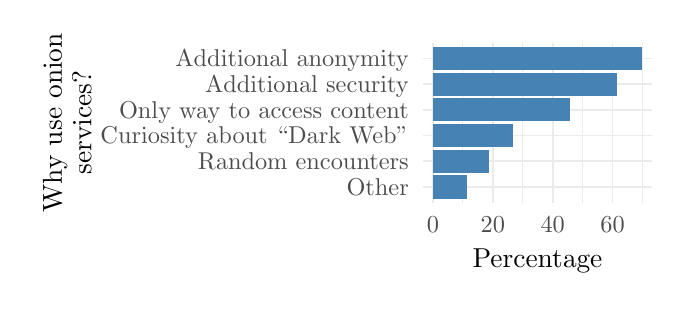
\begin{tikzpicture}[x=1pt,y=1pt]
\definecolor{fillColor}{RGB}{255,255,255}
\path[use as bounding box,fill=fillColor,fill opacity=0.00] (0,0) rectangle (231.26, 93.95);
\begin{scope}
\path[clip] (142.68, 30.77) rectangle (225.76, 88.45);
\definecolor{drawColor}{gray}{0.92}

\path[draw=drawColor,line width= 0.3pt,line join=round] (157.27, 30.77) --
	(157.27, 88.45);

\path[draw=drawColor,line width= 0.3pt,line join=round] (178.90, 30.77) --
	(178.90, 88.45);

\path[draw=drawColor,line width= 0.3pt,line join=round] (200.54, 30.77) --
	(200.54, 88.45);

\path[draw=drawColor,line width= 0.3pt,line join=round] (222.17, 30.77) --
	(222.17, 88.45);

\path[draw=drawColor,line width= 0.6pt,line join=round] (142.68, 36.35) --
	(225.76, 36.35);

\path[draw=drawColor,line width= 0.6pt,line join=round] (142.68, 45.66) --
	(225.76, 45.66);

\path[draw=drawColor,line width= 0.6pt,line join=round] (142.68, 54.96) --
	(225.76, 54.96);

\path[draw=drawColor,line width= 0.6pt,line join=round] (142.68, 64.26) --
	(225.76, 64.26);

\path[draw=drawColor,line width= 0.6pt,line join=round] (142.68, 73.57) --
	(225.76, 73.57);

\path[draw=drawColor,line width= 0.6pt,line join=round] (142.68, 82.87) --
	(225.76, 82.87);

\path[draw=drawColor,line width= 0.6pt,line join=round] (146.45, 30.77) --
	(146.45, 88.45);

\path[draw=drawColor,line width= 0.6pt,line join=round] (168.09, 30.77) --
	(168.09, 88.45);

\path[draw=drawColor,line width= 0.6pt,line join=round] (189.72, 30.77) --
	(189.72, 88.45);

\path[draw=drawColor,line width= 0.6pt,line join=round] (211.35, 30.77) --
	(211.35, 88.45);
\definecolor{fillColor}{RGB}{70,130,180}

\path[fill=fillColor] (146.45, 32.17) rectangle (158.77, 40.54);

\path[fill=fillColor] (146.45, 41.47) rectangle (166.57, 49.84);

\path[fill=fillColor] (146.45, 50.77) rectangle (175.40, 59.15);

\path[fill=fillColor] (146.45, 60.08) rectangle (196.12, 68.45);

\path[fill=fillColor] (146.45, 69.38) rectangle (212.96, 77.75);

\path[fill=fillColor] (146.45, 78.68) rectangle (221.99, 87.06);
\end{scope}
\begin{scope}
\path[clip] (  0.00,  0.00) rectangle (231.26, 93.95);
\definecolor{drawColor}{gray}{0.30}

\node[text=drawColor,anchor=base east,inner sep=0pt, outer sep=0pt, scale=  0.88] at (137.73, 33.32) {Other};

\node[text=drawColor,anchor=base east,inner sep=0pt, outer sep=0pt, scale=  0.88] at (137.73, 42.63) {Random encounters};

\node[text=drawColor,anchor=base east,inner sep=0pt, outer sep=0pt, scale=  0.88] at (137.73, 51.93) {Curiosity about ``Dark Web''};

\node[text=drawColor,anchor=base east,inner sep=0pt, outer sep=0pt, scale=  0.88] at (137.73, 61.23) {Only way to access content};

\node[text=drawColor,anchor=base east,inner sep=0pt, outer sep=0pt, scale=  0.88] at (137.73, 70.54) {Additional security};

\node[text=drawColor,anchor=base east,inner sep=0pt, outer sep=0pt, scale=  0.88] at (137.73, 79.84) {Additional anonymity};
\end{scope}
\begin{scope}
\path[clip] (  0.00,  0.00) rectangle (231.26, 93.95);
\definecolor{drawColor}{gray}{0.30}

\node[text=drawColor,anchor=base,inner sep=0pt, outer sep=0pt, scale=  0.88] at (146.45, 19.76) {0};

\node[text=drawColor,anchor=base,inner sep=0pt, outer sep=0pt, scale=  0.88] at (168.09, 19.76) {20};

\node[text=drawColor,anchor=base,inner sep=0pt, outer sep=0pt, scale=  0.88] at (189.72, 19.76) {40};

\node[text=drawColor,anchor=base,inner sep=0pt, outer sep=0pt, scale=  0.88] at (211.35, 19.76) {60};
\end{scope}
\begin{scope}
\path[clip] (  0.00,  0.00) rectangle (231.26, 93.95);
\definecolor{drawColor}{RGB}{0,0,0}

\node[text=drawColor,anchor=base,inner sep=0pt, outer sep=0pt, scale=  0.99] at (184.22,  7.44) {Percentage};
\end{scope}
\begin{scope}
\path[clip] (  0.00,  0.00) rectangle (231.26, 93.95);
\definecolor{drawColor}{RGB}{0,0,0}

\node[text=drawColor,rotate= 90.00,anchor=base,inner sep=0pt, outer sep=0pt, scale=  0.99] at ( 12.32, 59.61) {Why use onion};

\node[text=drawColor,rotate= 90.00,anchor=base,inner sep=0pt, outer sep=0pt, scale=  0.99] at ( 23.01, 59.61) {services?};
\end{scope}
\end{tikzpicture}

    \caption{Our respondents' (multiple choice) reasons for using onion
    services.}
    \label{fig:onion-usage}
\end{figure}


\subsubsection{Misunderstanding of onion links and anonymity}
An unrelated, yet hardly unexpected, source of confusion amongst our survey respondents was the domain format of
onion services.  Some users believed that the seemingly-random
characters in onion domains are the reason why onion services are anonymous:

\begin{displayquote}[Survey respondent]
\ldots [The] Onion Services stay anonymous through changing their domain, and I
feel that there is a possibility of decreased anonymity with a constant domain
name.
\end{displayquote}

Accordingly, these users also believe that vanity domains \mc{do we explain what a vanity domain is earlier in the paper?} are ``less anonymous''
because part of their domains is clearly not random.  A survey participant
further wrote: \textquote{I understand vanity onion domains are a sign of the
weakness of the hash algorithm used by the Tor network.}  An unrelated yet
equally incorrect opinion was voiced by a different survey respondent:
\textquote{These people who created their onion name using scallion or other
tools should notice that other people can make same private key.}

\subsubsection{Reasons for Setting Up An Onion Service}
We asked if any participants operated an onion service, including the motivation for
running an onion service and what sort of issues operators encounter in the
process.  40\% of our survey respondents had once set up an onion service sometime in the past.  Among the survey
respondents who never had set up an onion service, 31\% have considered doing so while 30\% have never
considered it.  Interestingly, 79\% of the survey respondents who had set up onion services of their own had run their onion service for
private use while 53\% had run them for the public.

\Cref{fig:onion-operation-reasons} gives an overview of the reasons our
respondents have for running onion services.  Interestingly, the extra security
properties outweigh the anonymity properties of onion services.  Another popular
motivation is \textsc{nat} traversal---many respondents noted that onion
services allow them to expose a \textsc{tcp} service in their home network
despite being behind a \textsc{nat} device.  Finally, some people run onion
services indirectly because third-party tools such as
OnionShare~\cite{onionshare} or Ricochet~\cite{ricochet} are built on top of
them.  A survey respondent gave the following reason for running onion services:
\textquote{We use it for delivering updates to our router to customers securely
and without leaking metadata.}

\begin{figure}[t]
    \centering
    % Created by tikzDevice version 0.10.1 on 2018-01-12 16:24:46
% !TEX encoding = UTF-8 Unicode
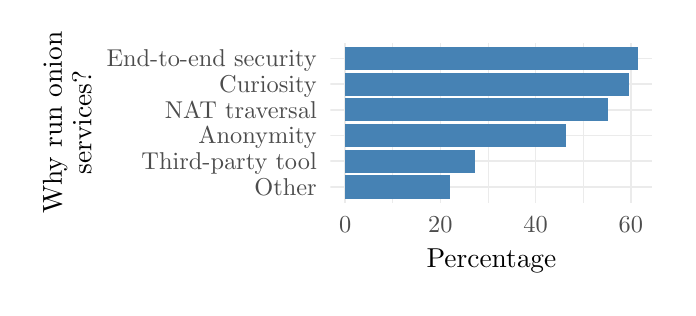
\begin{tikzpicture}[x=1pt,y=1pt]
\definecolor{fillColor}{RGB}{255,255,255}
\path[use as bounding box,fill=fillColor,fill opacity=0.00] (0,0) rectangle (231.26, 93.95);
\begin{scope}
\path[clip] (109.42, 30.77) rectangle (225.76, 88.45);
\definecolor{drawColor}{gray}{0.92}

\path[draw=drawColor,line width= 0.3pt,line join=round] (131.91, 30.77) --
	(131.91, 88.45);

\path[draw=drawColor,line width= 0.3pt,line join=round] (166.33, 30.77) --
	(166.33, 88.45);

\path[draw=drawColor,line width= 0.3pt,line join=round] (200.75, 30.77) --
	(200.75, 88.45);

\path[draw=drawColor,line width= 0.6pt,line join=round] (109.42, 36.35) --
	(225.76, 36.35);

\path[draw=drawColor,line width= 0.6pt,line join=round] (109.42, 45.66) --
	(225.76, 45.66);

\path[draw=drawColor,line width= 0.6pt,line join=round] (109.42, 54.96) --
	(225.76, 54.96);

\path[draw=drawColor,line width= 0.6pt,line join=round] (109.42, 64.26) --
	(225.76, 64.26);

\path[draw=drawColor,line width= 0.6pt,line join=round] (109.42, 73.57) --
	(225.76, 73.57);

\path[draw=drawColor,line width= 0.6pt,line join=round] (109.42, 82.87) --
	(225.76, 82.87);

\path[draw=drawColor,line width= 0.6pt,line join=round] (114.70, 30.77) --
	(114.70, 88.45);

\path[draw=drawColor,line width= 0.6pt,line join=round] (149.12, 30.77) --
	(149.12, 88.45);

\path[draw=drawColor,line width= 0.6pt,line join=round] (183.54, 30.77) --
	(183.54, 88.45);

\path[draw=drawColor,line width= 0.6pt,line join=round] (217.96, 30.77) --
	(217.96, 88.45);
\definecolor{fillColor}{RGB}{70,130,180}

\path[fill=fillColor] (114.70, 32.17) rectangle (152.48, 40.54);

\path[fill=fillColor] (114.70, 41.47) rectangle (161.72, 49.84);

\path[fill=fillColor] (114.70, 50.77) rectangle (194.45, 59.15);

\path[fill=fillColor] (114.70, 60.08) rectangle (209.56, 68.45);

\path[fill=fillColor] (114.70, 69.38) rectangle (217.12, 77.75);

\path[fill=fillColor] (114.70, 78.68) rectangle (220.48, 87.06);
\end{scope}
\begin{scope}
\path[clip] (  0.00,  0.00) rectangle (231.26, 93.95);
\definecolor{drawColor}{gray}{0.30}

\node[text=drawColor,anchor=base east,inner sep=0pt, outer sep=0pt, scale=  0.88] at (104.47, 33.32) {Other};

\node[text=drawColor,anchor=base east,inner sep=0pt, outer sep=0pt, scale=  0.88] at (104.47, 42.63) {Third-party tool};

\node[text=drawColor,anchor=base east,inner sep=0pt, outer sep=0pt, scale=  0.88] at (104.47, 51.93) {Anonymity};

\node[text=drawColor,anchor=base east,inner sep=0pt, outer sep=0pt, scale=  0.88] at (104.47, 61.23) {NAT traversal};

\node[text=drawColor,anchor=base east,inner sep=0pt, outer sep=0pt, scale=  0.88] at (104.47, 70.54) {Curiosity};

\node[text=drawColor,anchor=base east,inner sep=0pt, outer sep=0pt, scale=  0.88] at (104.47, 79.84) {End-to-end security};
\end{scope}
\begin{scope}
\path[clip] (  0.00,  0.00) rectangle (231.26, 93.95);
\definecolor{drawColor}{gray}{0.30}

\node[text=drawColor,anchor=base,inner sep=0pt, outer sep=0pt, scale=  0.88] at (114.70, 19.76) {0};

\node[text=drawColor,anchor=base,inner sep=0pt, outer sep=0pt, scale=  0.88] at (149.12, 19.76) {20};

\node[text=drawColor,anchor=base,inner sep=0pt, outer sep=0pt, scale=  0.88] at (183.54, 19.76) {40};

\node[text=drawColor,anchor=base,inner sep=0pt, outer sep=0pt, scale=  0.88] at (217.96, 19.76) {60};
\end{scope}
\begin{scope}
\path[clip] (  0.00,  0.00) rectangle (231.26, 93.95);
\definecolor{drawColor}{RGB}{0,0,0}

\node[text=drawColor,anchor=base,inner sep=0pt, outer sep=0pt, scale=  0.99] at (167.59,  7.44) {Percentage};
\end{scope}
\begin{scope}
\path[clip] (  0.00,  0.00) rectangle (231.26, 93.95);
\definecolor{drawColor}{RGB}{0,0,0}

\node[text=drawColor,rotate= 90.00,anchor=base,inner sep=0pt, outer sep=0pt, scale=  0.99] at ( 12.32, 59.61) {Why run onion};

\node[text=drawColor,rotate= 90.00,anchor=base,inner sep=0pt, outer sep=0pt, scale=  0.99] at ( 23.01, 59.61) {services?};
\end{scope}
\end{tikzpicture}

    \caption{The (multiple-choice) reasons our respondents have for running
    onion services.}
    \label{fig:onion-operation-reasons}
\end{figure}

\subsection{Onion service discovery \& management}
\label{sec:manage}

\subsubsection{Onion links usually discovered on social media, on the web, or via search engines }
Recall that a freshly set up onion service is private by default, leaving it up
to its operator to disseminate the domain.  Established search engines such as
Google are therefore inadequate to find content on onion services.  We wanted to
find out how our survey respondents discover onion services.
\Cref{fig:onion-discovery} illustrates the results.  The three most popular ways
that participants discovered new onion sites, all approximating 50\%, were via \first~social
networking sites such as Twitter and Reddit, \second~the list of search engines
such as Ahmia,\footnote{Ahmia.fi is an onion site search engine that crawls
user-submitted onion domains.  It publishes the list of all indexed onion
services at \url{https://ahmia.fi/onions/}.} and \third~randomly encountering
links when browsing the web.

While significantly less popular, participants told us that discovering onion domains through friends and
family had the advantage that domains come from a trusted source---an aspect
that mattered to some of our survey and interview participants.  Finally, a mere
4\% of our survey respondents indicated that they were not interested in learning about new onion services.
Respondents who selected ``Other'' predominantly brought up
independently-maintained onion domain aggregators.  A noteworthy example is the
Hidden Wiki, a community-curated and frequently-forked wiki that contains
categorized links to onion services.

\begin{figure}[t]
    \centering
    % Created by tikzDevice version 0.10.1 on 2018-01-12 16:15:03
% !TEX encoding = UTF-8 Unicode
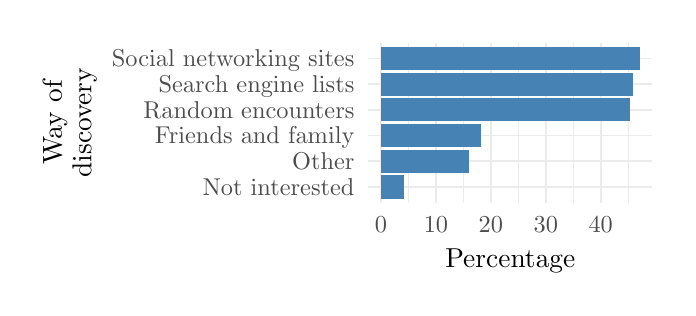
\begin{tikzpicture}[x=1pt,y=1pt]
\definecolor{fillColor}{RGB}{255,255,255}
\path[use as bounding box,fill=fillColor,fill opacity=0.00] (0,0) rectangle (231.26, 93.95);
\begin{scope}
\path[clip] (123.02, 30.77) rectangle (225.76, 88.45);
\definecolor{drawColor}{gray}{0.92}

\path[draw=drawColor,line width= 0.3pt,line join=round] (137.61, 30.77) --
	(137.61, 88.45);

\path[draw=drawColor,line width= 0.3pt,line join=round] (157.46, 30.77) --
	(157.46, 88.45);

\path[draw=drawColor,line width= 0.3pt,line join=round] (177.31, 30.77) --
	(177.31, 88.45);

\path[draw=drawColor,line width= 0.3pt,line join=round] (197.16, 30.77) --
	(197.16, 88.45);

\path[draw=drawColor,line width= 0.3pt,line join=round] (217.00, 30.77) --
	(217.00, 88.45);

\path[draw=drawColor,line width= 0.6pt,line join=round] (123.02, 36.35) --
	(225.76, 36.35);

\path[draw=drawColor,line width= 0.6pt,line join=round] (123.02, 45.66) --
	(225.76, 45.66);

\path[draw=drawColor,line width= 0.6pt,line join=round] (123.02, 54.96) --
	(225.76, 54.96);

\path[draw=drawColor,line width= 0.6pt,line join=round] (123.02, 64.26) --
	(225.76, 64.26);

\path[draw=drawColor,line width= 0.6pt,line join=round] (123.02, 73.57) --
	(225.76, 73.57);

\path[draw=drawColor,line width= 0.6pt,line join=round] (123.02, 82.87) --
	(225.76, 82.87);

\path[draw=drawColor,line width= 0.6pt,line join=round] (127.69, 30.77) --
	(127.69, 88.45);

\path[draw=drawColor,line width= 0.6pt,line join=round] (147.54, 30.77) --
	(147.54, 88.45);

\path[draw=drawColor,line width= 0.6pt,line join=round] (167.38, 30.77) --
	(167.38, 88.45);

\path[draw=drawColor,line width= 0.6pt,line join=round] (187.23, 30.77) --
	(187.23, 88.45);

\path[draw=drawColor,line width= 0.6pt,line join=round] (207.08, 30.77) --
	(207.08, 88.45);
\definecolor{fillColor}{RGB}{70,130,180}

\path[fill=fillColor] (127.69, 32.17) rectangle (135.96, 40.54);

\path[fill=fillColor] (127.69, 41.47) rectangle (159.33, 49.84);

\path[fill=fillColor] (127.69, 50.77) rectangle (163.85, 59.15);

\path[fill=fillColor] (127.69, 60.08) rectangle (217.70, 68.45);

\path[fill=fillColor] (127.69, 69.38) rectangle (218.83, 77.75);

\path[fill=fillColor] (127.69, 78.68) rectangle (221.09, 87.06);
\end{scope}
\begin{scope}
\path[clip] (  0.00,  0.00) rectangle (231.26, 93.95);
\definecolor{drawColor}{gray}{0.30}

\node[text=drawColor,anchor=base east,inner sep=0pt, outer sep=0pt, scale=  0.88] at (118.07, 33.32) {Not interested};

\node[text=drawColor,anchor=base east,inner sep=0pt, outer sep=0pt, scale=  0.88] at (118.07, 42.63) {Other};

\node[text=drawColor,anchor=base east,inner sep=0pt, outer sep=0pt, scale=  0.88] at (118.07, 51.93) {Friends and family};

\node[text=drawColor,anchor=base east,inner sep=0pt, outer sep=0pt, scale=  0.88] at (118.07, 61.23) {Random encounters};

\node[text=drawColor,anchor=base east,inner sep=0pt, outer sep=0pt, scale=  0.88] at (118.07, 70.54) {Search engine lists};

\node[text=drawColor,anchor=base east,inner sep=0pt, outer sep=0pt, scale=  0.88] at (118.07, 79.84) {Social networking sites};
\end{scope}
\begin{scope}
\path[clip] (  0.00,  0.00) rectangle (231.26, 93.95);
\definecolor{drawColor}{gray}{0.30}

\node[text=drawColor,anchor=base,inner sep=0pt, outer sep=0pt, scale=  0.88] at (127.69, 19.76) {0};

\node[text=drawColor,anchor=base,inner sep=0pt, outer sep=0pt, scale=  0.88] at (147.54, 19.76) {10};

\node[text=drawColor,anchor=base,inner sep=0pt, outer sep=0pt, scale=  0.88] at (167.38, 19.76) {20};

\node[text=drawColor,anchor=base,inner sep=0pt, outer sep=0pt, scale=  0.88] at (187.23, 19.76) {30};

\node[text=drawColor,anchor=base,inner sep=0pt, outer sep=0pt, scale=  0.88] at (207.08, 19.76) {40};
\end{scope}
\begin{scope}
\path[clip] (  0.00,  0.00) rectangle (231.26, 93.95);
\definecolor{drawColor}{RGB}{0,0,0}

\node[text=drawColor,anchor=base,inner sep=0pt, outer sep=0pt, scale=  0.99] at (174.39,  7.44) {Percentage};
\end{scope}
\begin{scope}
\path[clip] (  0.00,  0.00) rectangle (231.26, 93.95);
\definecolor{drawColor}{RGB}{0,0,0}

\node[text=drawColor,rotate= 90.00,anchor=base,inner sep=0pt, outer sep=0pt, scale=  0.99] at ( 12.32, 59.61) {Way of};

\node[text=drawColor,rotate= 90.00,anchor=base,inner sep=0pt, outer sep=0pt, scale=  0.99] at ( 23.01, 59.61) {discovery};
\end{scope}
\end{tikzpicture}

    \caption{Our respondents' (multiple choice) methods of discovering onion
    services.}
    \label{fig:onion-discovery}
\end{figure}

The majority of our survey respondents (60\%) reported that they were satisfied with how they discover onion services but a significant proportion (40\%) were not. Those who were satisfied with how they discover onion links reported that they have no
interest in learning about new onion services, in part because they only use a
small set of onion services.  Among the survey respondents who were not satisfied, the most
prominent complaint was about link rot on aggregators.  There is significant
churn among onion sites, and our respondents were frustrated that aggregators
are typically not curated and therefore link to numerous dead domains.  The lack
of curation also leads to these aggregators' containing the occasional scam and
phishing site.  The difficulty of telling apart two given onion domain names
exacerbates this issue for users.  Another common wish for aggregators was for
them to be more verbose in their description of onion sites.  In particular,
some survey respondents wanted to avoid illegal and pornographic content, which is often
difficult if the description is vague and the onion domain reveals nothing about
its content.  Many survey respondents were not aware of search engines such as Ahmia.
Among those survey respondents that were aware of such engines, many were dissatisfied with both the search results and
the number of indexed onion sites.  Unsurprisingly, a ``Google for onion sites''
was a frequent wish.

Many survey respondents expressed frustration about the difficulty of finding out if a particular website, such as 
``example.com'' has a corresponding onion service.  A common wish was to have
a website list its onion service prominently in a footer.  Ironically, some
survey respondents were surprised that torproject.org has a corresponding onion
site---they could not find it on the web site.



\begin{figure}[t]
    \centering
    % Created by tikzDevice version 0.10.1 on 2018-02-09 14:36:33
% !TEX encoding = UTF-8 Unicode
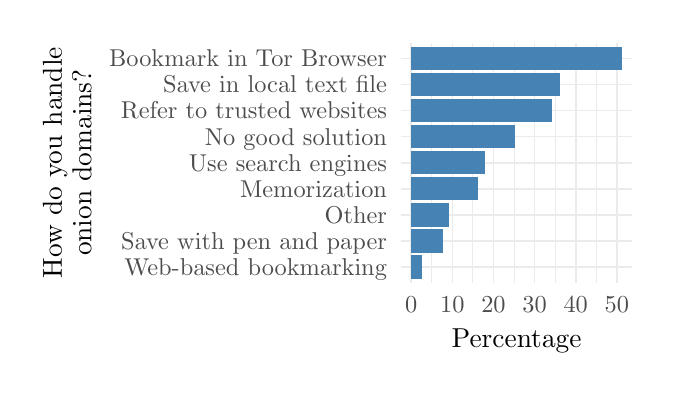
\begin{tikzpicture}[x=1pt,y=1pt]
\definecolor{fillColor}{RGB}{255,255,255}
\path[use as bounding box,fill=fillColor,fill opacity=0.00] (0,0) rectangle (224.04,122.86);
\begin{scope}
\path[clip] (134.78, 30.77) rectangle (218.54,117.36);
\definecolor{drawColor}{gray}{0.92}

\path[draw=drawColor,line width= 0.3pt,line join=round] (146.02, 30.77) --
	(146.02,117.36);

\path[draw=drawColor,line width= 0.3pt,line join=round] (160.88, 30.77) --
	(160.88,117.36);

\path[draw=drawColor,line width= 0.3pt,line join=round] (175.74, 30.77) --
	(175.74,117.36);

\path[draw=drawColor,line width= 0.3pt,line join=round] (190.61, 30.77) --
	(190.61,117.36);

\path[draw=drawColor,line width= 0.3pt,line join=round] (205.47, 30.77) --
	(205.47,117.36);

\path[draw=drawColor,line width= 0.6pt,line join=round] (134.78, 36.42) --
	(218.54, 36.42);

\path[draw=drawColor,line width= 0.6pt,line join=round] (134.78, 45.83) --
	(218.54, 45.83);

\path[draw=drawColor,line width= 0.6pt,line join=round] (134.78, 55.24) --
	(218.54, 55.24);

\path[draw=drawColor,line width= 0.6pt,line join=round] (134.78, 64.65) --
	(218.54, 64.65);

\path[draw=drawColor,line width= 0.6pt,line join=round] (134.78, 74.07) --
	(218.54, 74.07);

\path[draw=drawColor,line width= 0.6pt,line join=round] (134.78, 83.48) --
	(218.54, 83.48);

\path[draw=drawColor,line width= 0.6pt,line join=round] (134.78, 92.89) --
	(218.54, 92.89);

\path[draw=drawColor,line width= 0.6pt,line join=round] (134.78,102.30) --
	(218.54,102.30);

\path[draw=drawColor,line width= 0.6pt,line join=round] (134.78,111.71) --
	(218.54,111.71);

\path[draw=drawColor,line width= 0.6pt,line join=round] (138.58, 30.77) --
	(138.58,117.36);

\path[draw=drawColor,line width= 0.6pt,line join=round] (153.45, 30.77) --
	(153.45,117.36);

\path[draw=drawColor,line width= 0.6pt,line join=round] (168.31, 30.77) --
	(168.31,117.36);

\path[draw=drawColor,line width= 0.6pt,line join=round] (183.17, 30.77) --
	(183.17,117.36);

\path[draw=drawColor,line width= 0.6pt,line join=round] (198.04, 30.77) --
	(198.04,117.36);

\path[draw=drawColor,line width= 0.6pt,line join=round] (212.90, 30.77) --
	(212.90,117.36);
\definecolor{fillColor}{RGB}{70,130,180}

\path[fill=fillColor] (138.58, 32.18) rectangle (142.54, 40.66);

\path[fill=fillColor] (138.58, 41.60) rectangle (150.15, 50.07);

\path[fill=fillColor] (138.58, 51.01) rectangle (152.13, 59.48);

\path[fill=fillColor] (138.58, 60.42) rectangle (162.84, 68.89);

\path[fill=fillColor] (138.58, 69.83) rectangle (165.10, 78.30);

\path[fill=fillColor] (138.58, 79.24) rectangle (176.10, 87.71);

\path[fill=fillColor] (138.58, 88.65) rectangle (189.36, 97.12);

\path[fill=fillColor] (138.58, 98.07) rectangle (192.45,106.54);

\path[fill=fillColor] (138.58,107.48) rectangle (214.73,115.95);
\end{scope}
\begin{scope}
\path[clip] (  0.00,  0.00) rectangle (224.04,122.86);
\definecolor{drawColor}{gray}{0.30}

\node[text=drawColor,anchor=base east,inner sep=0pt, outer sep=0pt, scale=  0.88] at (129.83, 33.39) {Web-based bookmarking};

\node[text=drawColor,anchor=base east,inner sep=0pt, outer sep=0pt, scale=  0.88] at (129.83, 42.80) {Save with pen and paper};

\node[text=drawColor,anchor=base east,inner sep=0pt, outer sep=0pt, scale=  0.88] at (129.83, 52.21) {Other};

\node[text=drawColor,anchor=base east,inner sep=0pt, outer sep=0pt, scale=  0.88] at (129.83, 61.62) {Memorization};

\node[text=drawColor,anchor=base east,inner sep=0pt, outer sep=0pt, scale=  0.88] at (129.83, 71.04) {Use search engines};

\node[text=drawColor,anchor=base east,inner sep=0pt, outer sep=0pt, scale=  0.88] at (129.83, 80.45) {No good solution};

\node[text=drawColor,anchor=base east,inner sep=0pt, outer sep=0pt, scale=  0.88] at (129.83, 89.86) {Refer to trusted websites};

\node[text=drawColor,anchor=base east,inner sep=0pt, outer sep=0pt, scale=  0.88] at (129.83, 99.27) {Save in local text file};

\node[text=drawColor,anchor=base east,inner sep=0pt, outer sep=0pt, scale=  0.88] at (129.83,108.68) {Bookmark in Tor Browser};
\end{scope}
\begin{scope}
\path[clip] (  0.00,  0.00) rectangle (224.04,122.86);
\definecolor{drawColor}{gray}{0.30}

\node[text=drawColor,anchor=base,inner sep=0pt, outer sep=0pt, scale=  0.88] at (138.58, 19.76) {0};

\node[text=drawColor,anchor=base,inner sep=0pt, outer sep=0pt, scale=  0.88] at (153.45, 19.76) {10};

\node[text=drawColor,anchor=base,inner sep=0pt, outer sep=0pt, scale=  0.88] at (168.31, 19.76) {20};

\node[text=drawColor,anchor=base,inner sep=0pt, outer sep=0pt, scale=  0.88] at (183.17, 19.76) {30};

\node[text=drawColor,anchor=base,inner sep=0pt, outer sep=0pt, scale=  0.88] at (198.04, 19.76) {40};

\node[text=drawColor,anchor=base,inner sep=0pt, outer sep=0pt, scale=  0.88] at (212.90, 19.76) {50};
\end{scope}
\begin{scope}
\path[clip] (  0.00,  0.00) rectangle (224.04,122.86);
\definecolor{drawColor}{RGB}{0,0,0}

\node[text=drawColor,anchor=base,inner sep=0pt, outer sep=0pt, scale=  0.99] at (176.66,  7.44) {Percentage};
\end{scope}
\begin{scope}
\path[clip] (  0.00,  0.00) rectangle (224.04,122.86);
\definecolor{drawColor}{RGB}{0,0,0}

\node[text=drawColor,rotate= 90.00,anchor=base,inner sep=0pt, outer sep=0pt, scale=  0.99] at ( 12.32, 74.07) {How do you handle};

\node[text=drawColor,rotate= 90.00,anchor=base,inner sep=0pt, outer sep=0pt, scale=  0.99] at ( 23.01, 74.07) {onion domains?};
\end{scope}
\end{tikzpicture}

    \caption{The strategies that our respondents use to handle onion domains.
    More than half use bookmarks inside of Tor Browser and a quarter thinks that
    there is no good solution.}
    \label{fig:onion-domain-mgmt}
\end{figure}

\subsubsection{Saving and tracking onion links is not straightforward}
While conventional domains are designed to be easy to remember and recognize, we wanted to know how users handle randomly-generated onion domains. Most survey respondents use Tor Browser's bookmarks to save onion domains as seen in \Cref{fig:onion-domain-mgmt}.  While
convenient, this method of saving onion links leaves a trace of (presumably) visited sites on somebody's
computer.  One of Tor Browser's security requirements is ``disk avoidance,''
\ie, the browser must not write anything to disk that would reveal the user's
browsing history~\cite[\S~2.1]{Perry2017a}.  Bookmarking links is a violation of
this security requirement albeit requested by the user.  Many of our survey respondents
were aware of this issue, and about a dozen survey respondents who selected ``Other''
stated that they store onion domains in an encrypted manner---either in a text
file or in their password manager.  Somewhat less popular amongst our survey participants was saving onion
domains in local text files (36\%), getting them from trusted web sites (34\%),
using search engines (18\%), memorizing domains (16\%), using some other
techniques (9\%), or employing pen and paper (8\%).  Notably, one quarter of our survey
respondents did not have a good solution to the problem of tracking onion links.  Given the alarming
number of (possibly insecure) home-baked solutions, a Tor Browser extension that
solves this problem seems warranted.

Of the survey respondents who memorize onion domains, we found that most respondents
memorize one to four onion domains (35\% of total respondents) but only 1\% are able to memorize more than four domains (1\%).   Survey respondents memorized domains \first~automatically start to memorize domains
because of typing it many times (60\%)
\second~to allow them to open the site more
quickly (51\%), and \third~to ensure that they are visiting the correct site and
not a phishing site (44\%). Others were privacy conscious because as mentioned above,
bookmarking onion domains leaves a trace. These 28\% of survey respondents said
they memorized onion domains to prevent this digital trace.

\subsubsection{Vanity domains are easier to memorize and track}
The majority of our survey respondents appreciated vanity domains because they were easy
to remember (64\%) and easy to recognize (64\%), and they provided a unique
``branding'' (34\%).  Some survey respondents indicated that a vanity prefix---like a
traditional domain---informs about an onion service's content, letting visitors
know what to expect and thus preventing unpleasant surprises.  Only 8\% disliked
vanity onion domains, and 15\% did not have an opinion.  Interestingly, some survey
respondents consider vanity domains economically unfair because wealthy entities
can afford to generate longer prefixes such as Facebook \mc{explain why in related work}.  Several respondents also voiced their
concern that vanity domains create a false sense of security and facilitate
phishing attacks. \mc{how so? can we say more}




We asked survey respondents
about whether or not they memorize vanity domains---specifically
facebookcorewwwi.onion---and how difficult they find it to memorize onion
domains of differing levels of vanity.  59\% of respondents replied that
facebookcorewwwi.onion is among the sites that they have memorized.  This is \mc{what are the participant or survey respondent ids for the quotes}
because it is ``easy to memorize'' and ``after seeing [it] many times, I
automatically start to memorize it.'' Depending on the format of the vanity domain, our survey respondents expressed differing levels of ease for
memorizing them; these results are shown in \Cref{fig:memorize-domains}.
\textsc{Url}s such as expyuzz4wqqyqhjn.onion and torproz4wqqyqhjn.onion are
harder for respondents to remember because they mention that ``numbers make the
names harder to remember.''  Other survey respondents stated that vanity domains are easier to
remember when they can be pronounced.  One respondent described it saying \mc{need participant id}
``phonetic pronunciation plays a large part in how I remember onions.'' Many
other survey respondents stated that onion domains that are supported by a mnemonic are
also easier to remember.  

\begin{figure}[t]
    \centering
    % Created by tikzDevice version 0.10.1 on 2018-02-09 14:43:10
% !TEX encoding = UTF-8 Unicode
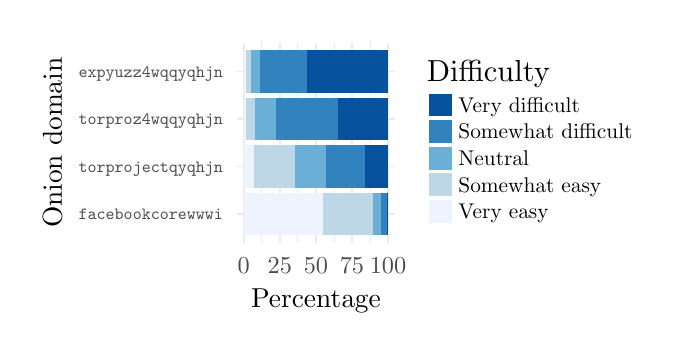
\begin{tikzpicture}[x=1pt,y=1pt]
\definecolor{fillColor}{RGB}{255,255,255}
\path[use as bounding box,fill=fillColor,fill opacity=0.00] (0,0) rectangle (224.04,108.41);
\begin{scope}
\path[clip] ( 75.47, 30.77) rectangle (132.84,102.91);
\definecolor{drawColor}{gray}{0.92}

\path[draw=drawColor,line width= 0.3pt,line join=round] ( 84.60, 30.77) --
	( 84.60,102.91);

\path[draw=drawColor,line width= 0.3pt,line join=round] ( 97.64, 30.77) --
	( 97.64,102.91);

\path[draw=drawColor,line width= 0.3pt,line join=round] (110.67, 30.77) --
	(110.67,102.91);

\path[draw=drawColor,line width= 0.3pt,line join=round] (123.71, 30.77) --
	(123.71,102.91);

\path[draw=drawColor,line width= 0.6pt,line join=round] ( 75.47, 41.08) --
	(132.84, 41.08);

\path[draw=drawColor,line width= 0.6pt,line join=round] ( 75.47, 58.25) --
	(132.84, 58.25);

\path[draw=drawColor,line width= 0.6pt,line join=round] ( 75.47, 75.43) --
	(132.84, 75.43);

\path[draw=drawColor,line width= 0.6pt,line join=round] ( 75.47, 92.60) --
	(132.84, 92.60);

\path[draw=drawColor,line width= 0.6pt,line join=round] ( 78.08, 30.77) --
	( 78.08,102.91);

\path[draw=drawColor,line width= 0.6pt,line join=round] ( 91.12, 30.77) --
	( 91.12,102.91);

\path[draw=drawColor,line width= 0.6pt,line join=round] (104.16, 30.77) --
	(104.16,102.91);

\path[draw=drawColor,line width= 0.6pt,line join=round] (117.19, 30.77) --
	(117.19,102.91);

\path[draw=drawColor,line width= 0.6pt,line join=round] (130.23, 30.77) --
	(130.23,102.91);
\definecolor{fillColor}{RGB}{239,243,255}

\path[fill=fillColor] ( 78.08, 33.35) rectangle (106.78, 48.81);
\definecolor{fillColor}{RGB}{189,215,231}

\path[fill=fillColor] (106.78, 33.35) rectangle (124.77, 48.81);
\definecolor{fillColor}{RGB}{107,174,214}

\path[fill=fillColor] (124.77, 33.35) rectangle (127.56, 48.81);
\definecolor{fillColor}{RGB}{49,130,189}

\path[fill=fillColor] (127.56, 33.35) rectangle (129.70, 48.81);
\definecolor{fillColor}{RGB}{8,81,156}

\path[fill=fillColor] (129.70, 33.35) rectangle (130.24, 48.81);
\definecolor{fillColor}{RGB}{239,243,255}

\path[fill=fillColor] ( 78.08, 50.52) rectangle ( 81.93, 65.98);
\definecolor{fillColor}{RGB}{189,215,231}

\path[fill=fillColor] ( 81.93, 50.52) rectangle ( 96.50, 65.98);
\definecolor{fillColor}{RGB}{107,174,214}

\path[fill=fillColor] ( 96.50, 50.52) rectangle (107.64, 65.98);
\definecolor{fillColor}{RGB}{49,130,189}

\path[fill=fillColor] (107.64, 50.52) rectangle (121.88, 65.98);
\definecolor{fillColor}{RGB}{8,81,156}

\path[fill=fillColor] (121.88, 50.52) rectangle (130.24, 65.98);
\definecolor{fillColor}{RGB}{239,243,255}

\path[fill=fillColor] ( 78.08, 67.70) rectangle ( 78.94, 83.15);
\definecolor{fillColor}{RGB}{189,215,231}

\path[fill=fillColor] ( 78.94, 67.70) rectangle ( 82.05, 83.15);
\definecolor{fillColor}{RGB}{107,174,214}

\path[fill=fillColor] ( 82.05, 67.70) rectangle ( 89.67, 83.15);
\definecolor{fillColor}{RGB}{49,130,189}

\path[fill=fillColor] ( 89.67, 67.70) rectangle (112.21, 83.15);
\definecolor{fillColor}{RGB}{8,81,156}

\path[fill=fillColor] (112.21, 67.70) rectangle (130.24, 83.15);
\definecolor{fillColor}{RGB}{239,243,255}

\path[fill=fillColor] ( 78.08, 84.87) rectangle ( 78.73,100.33);
\definecolor{fillColor}{RGB}{189,215,231}

\path[fill=fillColor] ( 78.73, 84.87) rectangle ( 80.78,100.33);
\definecolor{fillColor}{RGB}{107,174,214}

\path[fill=fillColor] ( 80.78, 84.87) rectangle ( 83.80,100.33);
\definecolor{fillColor}{RGB}{49,130,189}

\path[fill=fillColor] ( 83.80, 84.87) rectangle (100.82,100.33);
\definecolor{fillColor}{RGB}{8,81,156}

\path[fill=fillColor] (100.82, 84.87) rectangle (130.23,100.33);
\end{scope}
\begin{scope}
\path[clip] (  0.00,  0.00) rectangle (224.04,108.41);
\definecolor{drawColor}{gray}{0.30}

\node[text=drawColor,anchor=base east,inner sep=0pt, outer sep=0pt, scale=  0.62] at ( 70.52, 38.96) {\texttt{facebookcorewwwi}};

\node[text=drawColor,anchor=base east,inner sep=0pt, outer sep=0pt, scale=  0.62] at ( 70.52, 56.13) {\texttt{torprojectqyqhjn}};

\node[text=drawColor,anchor=base east,inner sep=0pt, outer sep=0pt, scale=  0.62] at ( 70.52, 73.30) {\texttt{torproz4wqqyqhjn}};

\node[text=drawColor,anchor=base east,inner sep=0pt, outer sep=0pt, scale=  0.62] at ( 70.52, 90.48) {\texttt{expyuzz4wqqyqhjn}};
\end{scope}
\begin{scope}
\path[clip] (  0.00,  0.00) rectangle (224.04,108.41);
\definecolor{drawColor}{gray}{0.30}

\node[text=drawColor,anchor=base,inner sep=0pt, outer sep=0pt, scale=  0.88] at ( 78.08, 19.76) {0};

\node[text=drawColor,anchor=base,inner sep=0pt, outer sep=0pt, scale=  0.88] at ( 91.12, 19.76) {25};

\node[text=drawColor,anchor=base,inner sep=0pt, outer sep=0pt, scale=  0.88] at (104.16, 19.76) {50};

\node[text=drawColor,anchor=base,inner sep=0pt, outer sep=0pt, scale=  0.88] at (117.19, 19.76) {75};

\node[text=drawColor,anchor=base,inner sep=0pt, outer sep=0pt, scale=  0.88] at (130.23, 19.76) {100};
\end{scope}
\begin{scope}
\path[clip] (  0.00,  0.00) rectangle (224.04,108.41);
\definecolor{drawColor}{RGB}{0,0,0}

\node[text=drawColor,anchor=base,inner sep=0pt, outer sep=0pt, scale=  0.99] at (104.16,  7.44) {Percentage};
\end{scope}
\begin{scope}
\path[clip] (  0.00,  0.00) rectangle (224.04,108.41);
\definecolor{drawColor}{RGB}{0,0,0}

\node[text=drawColor,rotate= 90.00,anchor=base,inner sep=0pt, outer sep=0pt, scale=  0.99] at ( 12.32, 66.84) {Onion domain};
\end{scope}
\begin{scope}
\path[clip] (  0.00,  0.00) rectangle (224.04,108.41);
\definecolor{drawColor}{RGB}{0,0,0}

\node[text=drawColor,anchor=base west,inner sep=0pt, outer sep=0pt, scale=  1.10] at (144.23, 88.95) {Difficulty};
\end{scope}
\begin{scope}
\path[clip] (  0.00,  0.00) rectangle (224.04,108.41);
\definecolor{fillColor}{RGB}{8,81,156}

\path[fill=fillColor] (144.94, 76.41) rectangle (153.15, 84.62);
\end{scope}
\begin{scope}
\path[clip] (  0.00,  0.00) rectangle (224.04,108.41);
\definecolor{fillColor}{RGB}{49,130,189}

\path[fill=fillColor] (144.94, 66.77) rectangle (153.15, 74.99);
\end{scope}
\begin{scope}
\path[clip] (  0.00,  0.00) rectangle (224.04,108.41);
\definecolor{fillColor}{RGB}{107,174,214}

\path[fill=fillColor] (144.94, 57.14) rectangle (153.15, 65.35);
\end{scope}
\begin{scope}
\path[clip] (  0.00,  0.00) rectangle (224.04,108.41);
\definecolor{fillColor}{RGB}{189,215,231}

\path[fill=fillColor] (144.94, 47.50) rectangle (153.15, 55.72);
\end{scope}
\begin{scope}
\path[clip] (  0.00,  0.00) rectangle (224.04,108.41);
\definecolor{fillColor}{RGB}{239,243,255}

\path[fill=fillColor] (144.94, 37.87) rectangle (153.15, 46.08);
\end{scope}
\begin{scope}
\path[clip] (  0.00,  0.00) rectangle (224.04,108.41);
\definecolor{drawColor}{RGB}{0,0,0}

\node[text=drawColor,anchor=base west,inner sep=0pt, outer sep=0pt, scale=  0.77] at (155.67, 77.86) {Very difficult};
\end{scope}
\begin{scope}
\path[clip] (  0.00,  0.00) rectangle (224.04,108.41);
\definecolor{drawColor}{RGB}{0,0,0}

\node[text=drawColor,anchor=base west,inner sep=0pt, outer sep=0pt, scale=  0.77] at (155.67, 68.23) {Somewhat difficult};
\end{scope}
\begin{scope}
\path[clip] (  0.00,  0.00) rectangle (224.04,108.41);
\definecolor{drawColor}{RGB}{0,0,0}

\node[text=drawColor,anchor=base west,inner sep=0pt, outer sep=0pt, scale=  0.77] at (155.67, 58.59) {Neutral};
\end{scope}
\begin{scope}
\path[clip] (  0.00,  0.00) rectangle (224.04,108.41);
\definecolor{drawColor}{RGB}{0,0,0}

\node[text=drawColor,anchor=base west,inner sep=0pt, outer sep=0pt, scale=  0.77] at (155.67, 48.96) {Somewhat easy};
\end{scope}
\begin{scope}
\path[clip] (  0.00,  0.00) rectangle (224.04,108.41);
\definecolor{drawColor}{RGB}{0,0,0}

\node[text=drawColor,anchor=base west,inner sep=0pt, outer sep=0pt, scale=  0.77] at (155.67, 39.32) {Very easy};
\end{scope}
\end{tikzpicture}

    \caption{The difficulty our respondents would expect to face when trying to
    memorize four onion domains.}
    \label{fig:memorize-domains}
\end{figure}

Interestingly, most (83\%) of our survey participants did not expect the
next-generation domain format to change their browsing habits because they treat onion domains as
opaque identifiers and handle these links via tools such as bookmarks.  For the 17\% who expressed concern over the next generation domain format \mc{can we define what this is?}, they felt that they would no longer be able to memorize even the small
number of onion domains (such as Facebook's) that they used.
 This suggests that although onion links are difficult to handle, usability may not worsen with the new domain format.

\subsubsection{Onion Services operations}
We asked our survey respondents if they had ever set up their own onion site and the issues they faced as reported in \Cref{fig:onion-operation-concerns}.  We asked about three potential attacks on onion services; \first~somebody setting up a
phishing site for the operator's site, \second~a denial-of-service attack, and
\third~a deanonymization attack.  More than half of our survey respondents who operated an onion service were at least
somewhat concerned about all of these attacks.  Almost 40\% of survey respondents claimed to be
extremely concerned about somebody deanonymizing their onion service.  Indeed,
many survey respondents lamented the difficulty of protecting onion services from
application-layer deanonymization attacks.  Matic \ea\ demonstrated some of
these issues in 2015~\cite{Matic2015a}.

\begin{figure}[t]
    \centering
    % Created by tikzDevice version 0.10.1 on 2018-02-09 14:59:34
% !TEX encoding = UTF-8 Unicode
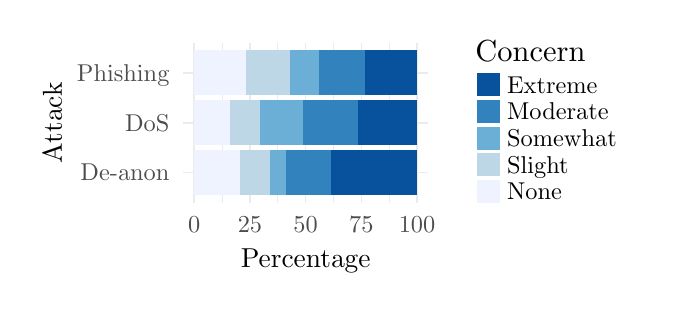
\begin{tikzpicture}[x=1pt,y=1pt]
\definecolor{fillColor}{RGB}{255,255,255}
\path[use as bounding box,fill=fillColor,fill opacity=0.00] (0,0) rectangle (224.04, 93.95);
\begin{scope}
\path[clip] ( 56.18, 30.77) rectangle (144.74, 88.45);
\definecolor{drawColor}{gray}{0.92}

\path[draw=drawColor,line width= 0.3pt,line join=round] ( 70.26, 30.77) --
	( 70.26, 88.45);

\path[draw=drawColor,line width= 0.3pt,line join=round] ( 90.39, 30.77) --
	( 90.39, 88.45);

\path[draw=drawColor,line width= 0.3pt,line join=round] (110.52, 30.77) --
	(110.52, 88.45);

\path[draw=drawColor,line width= 0.3pt,line join=round] (130.64, 30.77) --
	(130.64, 88.45);

\path[draw=drawColor,line width= 0.6pt,line join=round] ( 56.18, 41.59) --
	(144.74, 41.59);

\path[draw=drawColor,line width= 0.6pt,line join=round] ( 56.18, 59.61) --
	(144.74, 59.61);

\path[draw=drawColor,line width= 0.6pt,line join=round] ( 56.18, 77.64) --
	(144.74, 77.64);

\path[draw=drawColor,line width= 0.6pt,line join=round] ( 60.20, 30.77) --
	( 60.20, 88.45);

\path[draw=drawColor,line width= 0.6pt,line join=round] ( 80.33, 30.77) --
	( 80.33, 88.45);

\path[draw=drawColor,line width= 0.6pt,line join=round] (100.45, 30.77) --
	(100.45, 88.45);

\path[draw=drawColor,line width= 0.6pt,line join=round] (120.58, 30.77) --
	(120.58, 88.45);

\path[draw=drawColor,line width= 0.6pt,line join=round] (140.71, 30.77) --
	(140.71, 88.45);
\definecolor{fillColor}{RGB}{239,243,255}

\path[fill=fillColor] ( 60.20, 33.48) rectangle ( 76.78, 49.70);
\definecolor{fillColor}{RGB}{189,215,231}

\path[fill=fillColor] ( 76.78, 33.48) rectangle ( 87.44, 49.70);
\definecolor{fillColor}{RGB}{107,174,214}

\path[fill=fillColor] ( 87.44, 33.48) rectangle ( 93.35, 49.70);
\definecolor{fillColor}{RGB}{49,130,189}

\path[fill=fillColor] ( 93.35, 33.48) rectangle (109.54, 49.70);
\definecolor{fillColor}{RGB}{8,81,156}

\path[fill=fillColor] (109.54, 33.48) rectangle (140.72, 49.70);
\definecolor{fillColor}{RGB}{239,243,255}

\path[fill=fillColor] ( 60.20, 51.50) rectangle ( 73.16, 67.72);
\definecolor{fillColor}{RGB}{189,215,231}

\path[fill=fillColor] ( 73.16, 51.50) rectangle ( 83.77, 67.72);
\definecolor{fillColor}{RGB}{107,174,214}

\path[fill=fillColor] ( 83.77, 51.50) rectangle ( 99.47, 67.72);
\definecolor{fillColor}{RGB}{49,130,189}

\path[fill=fillColor] ( 99.47, 51.50) rectangle (119.50, 67.72);
\definecolor{fillColor}{RGB}{8,81,156}

\path[fill=fillColor] (119.50, 51.50) rectangle (140.71, 67.72);
\definecolor{fillColor}{RGB}{239,243,255}

\path[fill=fillColor] ( 60.20, 69.53) rectangle ( 79.05, 85.75);
\definecolor{fillColor}{RGB}{189,215,231}

\path[fill=fillColor] ( 79.05, 69.53) rectangle ( 94.75, 85.75);
\definecolor{fillColor}{RGB}{107,174,214}

\path[fill=fillColor] ( 94.75, 69.53) rectangle (105.36, 85.75);
\definecolor{fillColor}{RGB}{49,130,189}

\path[fill=fillColor] (105.36, 69.53) rectangle (121.85, 85.75);
\definecolor{fillColor}{RGB}{8,81,156}

\path[fill=fillColor] (121.85, 69.53) rectangle (140.70, 85.75);
\end{scope}
\begin{scope}
\path[clip] (  0.00,  0.00) rectangle (224.04, 93.95);
\definecolor{drawColor}{gray}{0.30}

\node[text=drawColor,anchor=base east,inner sep=0pt, outer sep=0pt, scale=  0.88] at ( 51.23, 38.56) {De-anon};

\node[text=drawColor,anchor=base east,inner sep=0pt, outer sep=0pt, scale=  0.88] at ( 51.23, 56.58) {DoS};

\node[text=drawColor,anchor=base east,inner sep=0pt, outer sep=0pt, scale=  0.88] at ( 51.23, 74.61) {Phishing};
\end{scope}
\begin{scope}
\path[clip] (  0.00,  0.00) rectangle (224.04, 93.95);
\definecolor{drawColor}{gray}{0.30}

\node[text=drawColor,anchor=base,inner sep=0pt, outer sep=0pt, scale=  0.88] at ( 60.20, 19.76) {0};

\node[text=drawColor,anchor=base,inner sep=0pt, outer sep=0pt, scale=  0.88] at ( 80.33, 19.76) {25};

\node[text=drawColor,anchor=base,inner sep=0pt, outer sep=0pt, scale=  0.88] at (100.45, 19.76) {50};

\node[text=drawColor,anchor=base,inner sep=0pt, outer sep=0pt, scale=  0.88] at (120.58, 19.76) {75};

\node[text=drawColor,anchor=base,inner sep=0pt, outer sep=0pt, scale=  0.88] at (140.71, 19.76) {100};
\end{scope}
\begin{scope}
\path[clip] (  0.00,  0.00) rectangle (224.04, 93.95);
\definecolor{drawColor}{RGB}{0,0,0}

\node[text=drawColor,anchor=base,inner sep=0pt, outer sep=0pt, scale=  0.99] at (100.46,  7.44) {Percentage};
\end{scope}
\begin{scope}
\path[clip] (  0.00,  0.00) rectangle (224.04, 93.95);
\definecolor{drawColor}{RGB}{0,0,0}

\node[text=drawColor,rotate= 90.00,anchor=base,inner sep=0pt, outer sep=0pt, scale=  0.99] at ( 12.32, 59.61) {Attack};
\end{scope}
\begin{scope}
\path[clip] (  0.00,  0.00) rectangle (224.04, 93.95);
\definecolor{drawColor}{RGB}{0,0,0}

\node[text=drawColor,anchor=base west,inner sep=0pt, outer sep=0pt, scale=  1.10] at (161.81, 81.72) {Concern};
\end{scope}
\begin{scope}
\path[clip] (  0.00,  0.00) rectangle (224.04, 93.95);
\definecolor{fillColor}{RGB}{8,81,156}

\path[fill=fillColor] (162.52, 69.18) rectangle (170.74, 77.40);
\end{scope}
\begin{scope}
\path[clip] (  0.00,  0.00) rectangle (224.04, 93.95);
\definecolor{fillColor}{RGB}{49,130,189}

\path[fill=fillColor] (162.52, 59.55) rectangle (170.74, 67.76);
\end{scope}
\begin{scope}
\path[clip] (  0.00,  0.00) rectangle (224.04, 93.95);
\definecolor{fillColor}{RGB}{107,174,214}

\path[fill=fillColor] (162.52, 49.91) rectangle (170.74, 58.12);
\end{scope}
\begin{scope}
\path[clip] (  0.00,  0.00) rectangle (224.04, 93.95);
\definecolor{fillColor}{RGB}{189,215,231}

\path[fill=fillColor] (162.52, 40.27) rectangle (170.74, 48.49);
\end{scope}
\begin{scope}
\path[clip] (  0.00,  0.00) rectangle (224.04, 93.95);
\definecolor{fillColor}{RGB}{239,243,255}

\path[fill=fillColor] (162.52, 30.64) rectangle (170.74, 38.85);
\end{scope}
\begin{scope}
\path[clip] (  0.00,  0.00) rectangle (224.04, 93.95);
\definecolor{drawColor}{RGB}{0,0,0}

\node[text=drawColor,anchor=base west,inner sep=0pt, outer sep=0pt, scale=  0.88] at (173.26, 70.26) {Extreme};
\end{scope}
\begin{scope}
\path[clip] (  0.00,  0.00) rectangle (224.04, 93.95);
\definecolor{drawColor}{RGB}{0,0,0}

\node[text=drawColor,anchor=base west,inner sep=0pt, outer sep=0pt, scale=  0.88] at (173.26, 60.62) {Moderate};
\end{scope}
\begin{scope}
\path[clip] (  0.00,  0.00) rectangle (224.04, 93.95);
\definecolor{drawColor}{RGB}{0,0,0}

\node[text=drawColor,anchor=base west,inner sep=0pt, outer sep=0pt, scale=  0.88] at (173.26, 50.99) {Somewhat};
\end{scope}
\begin{scope}
\path[clip] (  0.00,  0.00) rectangle (224.04, 93.95);
\definecolor{drawColor}{RGB}{0,0,0}

\node[text=drawColor,anchor=base west,inner sep=0pt, outer sep=0pt, scale=  0.88] at (173.26, 41.35) {Slight};
\end{scope}
\begin{scope}
\path[clip] (  0.00,  0.00) rectangle (224.04, 93.95);
\definecolor{drawColor}{RGB}{0,0,0}

\node[text=drawColor,anchor=base west,inner sep=0pt, outer sep=0pt, scale=  0.88] at (173.26, 31.71) {None};
\end{scope}
\end{tikzpicture}

    \caption{The level of concern onion service operators have with respect to a
    phishing clone of their service, denial-of-service attacks, and
    deanonymization.}
    \label{fig:onion-operation-concerns}
\end{figure}

\subsubsection{Onion links and sites are hard to verify as authentic}
We asked our survey respondents if they ever thought about the authenticity of an onion
site.  The majority of our survey respondents (80\%) did want to verify an onion service as authentic.  \Cref{fig:determining-legitimacy} gives an overview of the
strategies that our respondents employ.  More than half of our survey participants either consulted trusted
sources (\eg, friends or another, trusted web site) or used bookmarks when
revisiting onion services.  Many respondents also verified the domain in the
browser's address bar (46\%), checked if the corresponding web site had a link to
its onion site (41\%), or check that the onion service had an \textsc{https}
certificate (36\%).\footnote{DigiCert is issuing \textsc{ev} certificates for
onion sites~\cite{DigiCert2015a}, but adoption has been slow---presumably in part
because \textsc{ev} certificates require the \textsc{ca} to verify the
applicant's identity and they are not free.}  Alarmingly, almost 30\% of
survey respondents stated that they sometimes could not tell the difference between an
authentic service and an impersonation, and 11\% never checked a service's
legitimacy in the first place.  Survey participants who selected ``Other'' provided a wide
variety of ad-hoc phishing protections, some of which were clearly misguided, \mc{whats an example? and why was it misguided}
further highlighting the importance of being able to verify a site as being the one that they were trying to reach.

When asked how many characters our respondents verify in
onion domains,  43\% verified thirteen to sixteen digits, \ie, (almost) the full
domain, while 46\% verified up to nine digits, which is within the realm of brute
force attacks.

\begin{figure}[t]
    \centering
    % Created by tikzDevice version 0.10.1 on 2018-01-12 16:30:02
% !TEX encoding = UTF-8 Unicode
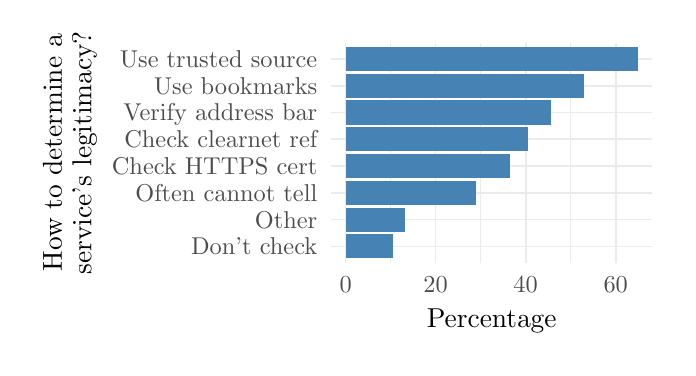
\begin{tikzpicture}[x=1pt,y=1pt]
\definecolor{fillColor}{RGB}{255,255,255}
\path[use as bounding box,fill=fillColor,fill opacity=0.00] (0,0) rectangle (231.26,115.63);
\begin{scope}
\path[clip] (109.60, 30.77) rectangle (225.76,110.13);
\definecolor{drawColor}{gray}{0.92}

\path[draw=drawColor,line width= 0.3pt,line join=round] (131.15, 30.77) --
	(131.15,110.13);

\path[draw=drawColor,line width= 0.3pt,line join=round] (163.68, 30.77) --
	(163.68,110.13);

\path[draw=drawColor,line width= 0.3pt,line join=round] (196.21, 30.77) --
	(196.21,110.13);

\path[draw=drawColor,line width= 0.6pt,line join=round] (109.60, 36.58) --
	(225.76, 36.58);

\path[draw=drawColor,line width= 0.6pt,line join=round] (109.60, 46.26) --
	(225.76, 46.26);

\path[draw=drawColor,line width= 0.6pt,line join=round] (109.60, 55.94) --
	(225.76, 55.94);

\path[draw=drawColor,line width= 0.6pt,line join=round] (109.60, 65.61) --
	(225.76, 65.61);

\path[draw=drawColor,line width= 0.6pt,line join=round] (109.60, 75.29) --
	(225.76, 75.29);

\path[draw=drawColor,line width= 0.6pt,line join=round] (109.60, 84.97) --
	(225.76, 84.97);

\path[draw=drawColor,line width= 0.6pt,line join=round] (109.60, 94.65) --
	(225.76, 94.65);

\path[draw=drawColor,line width= 0.6pt,line join=round] (109.60,104.33) --
	(225.76,104.33);

\path[draw=drawColor,line width= 0.6pt,line join=round] (114.88, 30.77) --
	(114.88,110.13);

\path[draw=drawColor,line width= 0.6pt,line join=round] (147.41, 30.77) --
	(147.41,110.13);

\path[draw=drawColor,line width= 0.6pt,line join=round] (179.95, 30.77) --
	(179.95,110.13);

\path[draw=drawColor,line width= 0.6pt,line join=round] (212.48, 30.77) --
	(212.48,110.13);
\definecolor{fillColor}{RGB}{70,130,180}

\path[fill=fillColor] (114.88, 32.22) rectangle (131.91, 40.93);

\path[fill=fillColor] (114.88, 41.90) rectangle (136.32, 50.61);

\path[fill=fillColor] (114.88, 51.58) rectangle (162.17, 60.29);

\path[fill=fillColor] (114.88, 61.26) rectangle (174.14, 69.97);

\path[fill=fillColor] (114.88, 70.94) rectangle (180.76, 79.65);

\path[fill=fillColor] (114.88, 80.61) rectangle (188.96, 89.32);

\path[fill=fillColor] (114.88, 90.29) rectangle (200.95, 99.00);

\path[fill=fillColor] (114.88, 99.97) rectangle (220.48,108.68);
\end{scope}
\begin{scope}
\path[clip] (  0.00,  0.00) rectangle (231.26,115.63);
\definecolor{drawColor}{gray}{0.30}

\node[text=drawColor,anchor=base east,inner sep=0pt, outer sep=0pt, scale=  0.88] at (104.65, 33.55) {Don't check};

\node[text=drawColor,anchor=base east,inner sep=0pt, outer sep=0pt, scale=  0.88] at (104.65, 43.23) {Other};

\node[text=drawColor,anchor=base east,inner sep=0pt, outer sep=0pt, scale=  0.88] at (104.65, 52.91) {Often cannot tell};

\node[text=drawColor,anchor=base east,inner sep=0pt, outer sep=0pt, scale=  0.88] at (104.65, 62.58) {Check HTTPS cert};

\node[text=drawColor,anchor=base east,inner sep=0pt, outer sep=0pt, scale=  0.88] at (104.65, 72.26) {Check clearnet ref};

\node[text=drawColor,anchor=base east,inner sep=0pt, outer sep=0pt, scale=  0.88] at (104.65, 81.94) {Verify address bar};

\node[text=drawColor,anchor=base east,inner sep=0pt, outer sep=0pt, scale=  0.88] at (104.65, 91.62) {Use bookmarks};

\node[text=drawColor,anchor=base east,inner sep=0pt, outer sep=0pt, scale=  0.88] at (104.65,101.29) {Use trusted source};
\end{scope}
\begin{scope}
\path[clip] (  0.00,  0.00) rectangle (231.26,115.63);
\definecolor{drawColor}{gray}{0.30}

\node[text=drawColor,anchor=base,inner sep=0pt, outer sep=0pt, scale=  0.88] at (114.88, 19.76) {0};

\node[text=drawColor,anchor=base,inner sep=0pt, outer sep=0pt, scale=  0.88] at (147.41, 19.76) {20};

\node[text=drawColor,anchor=base,inner sep=0pt, outer sep=0pt, scale=  0.88] at (179.95, 19.76) {40};

\node[text=drawColor,anchor=base,inner sep=0pt, outer sep=0pt, scale=  0.88] at (212.48, 19.76) {60};
\end{scope}
\begin{scope}
\path[clip] (  0.00,  0.00) rectangle (231.26,115.63);
\definecolor{drawColor}{RGB}{0,0,0}

\node[text=drawColor,anchor=base,inner sep=0pt, outer sep=0pt, scale=  0.99] at (167.68,  7.44) {Percentage};
\end{scope}
\begin{scope}
\path[clip] (  0.00,  0.00) rectangle (231.26,115.63);
\definecolor{drawColor}{RGB}{0,0,0}

\node[text=drawColor,rotate= 90.00,anchor=base,inner sep=0pt, outer sep=0pt, scale=  0.99] at ( 12.32, 70.45) {How to determine a};

\node[text=drawColor,rotate= 90.00,anchor=base,inner sep=0pt, outer sep=0pt, scale=  0.99] at ( 23.01, 70.45) {service's legitimacy?};
\end{scope}
\end{tikzpicture}

    \caption{How our respondents determine an onion service's legitimacy.}
    \label{fig:determining-legitimacy}
\end{figure}

Phishing remains an issue despite onion services' extra anonymity and security
properties.  Past work has documented phishing onion sites that transparently
rewrote Bitcoin addresses to hijack Bitcoin
transactions~\cite{Winter2016a,Nurmi2015a,Monteiro2016a}.  Key to this attack is
the difficulty of telling apart an authentic onion domain from an impersonation.
For conventional domains we rely on (\textsc{ev}) certificates, browser
protections, search results, and long-lived reputation, but none of these
methods have matured for onion services.  Does the nature of onion services
facilitate phishing attacks?  If so, what can we do to mitigate the issue?

Originally meant to provide ``branding'' for an onion service, vanity onion
domains also play a role in the context of phishing.  There is concern that the
short and recognizable prefixes tempt users to only verify the prefix and ignore
subsequent characters.  One respondent reported that \textquote{I only memorize
the first part of the domain.} \mc{need participant id} while another wrote:

\mc{need participant id}
\begin{displayquote}[Survey respondent]
If there isn't some cognizable word at the start, it'll be more difficult for me
to determine if I'm going to the correct domain or a scam. I may end up going to
less .onion sites as a result.
\end{displayquote}

Focusing only on the vanity part of a domain allows attackers to create an
impersonation domain that features the original's prefix but differs in
subsequent characters.  Nurmi~\cite{Nurmi2015a} and
Monteiro~\cite{Monteiro2016a} have both documented such an attack, but its
effectiveness is not known.


\subsection{Onion service issues \& improvements}
\label{sec:improve}

\subsubsection{Onion services are preferred for privacy reasons}
We asked our survey respondents if they would prefer onion versions of popular web sites such as
YouTube, Twitter, or Amazon to their normal web
sites. 49.07\% of survey respondents said they
would always prefer the onion site, 30.72\% chose ``Other'' and 20.21\% of
respondents said they would always prefer the normal web site,  Many of those
who selected ``Other'' had performance concerns. \mc{need participant id}  One user stated, ``I would
always prefer the onion site, but for video sites like YouTube I would likely
often use the normal site to be able to get a higher quality stream due to
higher bandwidth.'' Other survey respondents mentioned not wanting to log in to onion sites
because they believe it defeats the purpose by revealing private data---a fallacy that we discussed in
\Cref{sec:perception}.  In explaining their responses, survey respondents mentioned
that they like the privacy that onion sites provide, and they hoped that they
would not have to deal with \textsc{captcha}s and discrimination against Tor
users \mc{explain why this happens}.


We asked survey respondents if they would want Tor Browser to automatically redirect them from
a normal web site to its corresponding onion site (\eg, from facebook.com to
facebookcorewwwi.onion). Survey respondents were largely
in favor of this feature:37.78\% said they would always use it, 34.91\% said
they would use it for some sites, 15.61\% said they would never use that feature,   and
11.70\% chose ``Other.'' Survey respondents reported that they liked the convenience of being redirected.
The naysayers were quite passionate, though, and they were concerned about
potential security issues. One respondent said, \mc{participant id needed}
\textquote{What's to stop them from man in the middle'ing me, either by choice,
at the behest of some nefarious entity, or after being hacked?}
We conclude that there is clear interest in such an ``upgrade'' feature provided
that it is carefully designed and offers users an option to control the process
on a per-site basis.

